\documentclass{article}
\usepackage{geometry}
\geometry{
	a4paper,
	left=2.5cm,      % 左边距 2cm
	right=2.5cm,     % 右边距 2cm
	top=2.5cm,       % 上边距 2cm
	bottom=2.5cm,    % 下边距 2cm
	headheight=13.6pt
}
\usepackage{amsmath}
\usepackage{booktabs} % 用于三线表
\usepackage{caption}
\usepackage{setspace} % 用于设置行间距
\usepackage{array}
\usepackage{graphicx} % 用于插入图片
\usepackage{CTeX}
\setlength{\headheight}{13.6pt}
\usepackage{enumitem} % 用于自定义列表格式
\usepackage{svg}
\usepackage{pgfplots}
\pgfplotsset{compat=1.18}
\usepackage{palatino}  % 帕拉提诺体字体宏包
\usepackage{lipsum}  % 导入生成段落的宏包
\usepackage[hyperref=true,style=ieee]{biblatex}  % biblatex参考文献宏包
\usepackage{indentfirst}
\usepackage{booktabs} % For professional-looking tables
\usepackage{xcolor}   % For cell coloring
\usepackage{colortbl} % Required for \rowcolor
\definecolor{LightGreen}{rgb}{0.9, 0.95, 0.9}
\addbibresource{ref.bib}  % 添加引用文献bib源
\usepackage{fancyhdr}
\usepackage{enumitem} % 用于自定义列表格式
\usepackage{setspace}
\usepackage{svg}

\begin{document}
	\subsection{利用模拟退火算法优化xxx策略}
	
	\subsubsection{模拟退火算法模型分析}
	
	模拟退火算法是一种受固体退火过程启发的通用概率优化算法，用于在一个大的搜索空间中寻找给定问题的近似全局最优解。算法通过模仿物理中固体物质的退火过程优化策略，先将材料加热至高温，增加粒子动能，使其易于脱离局部能量最低态，再缓慢冷却，降低粒子动能，使其最终稳定在全局能量最低态，从而达到能量最低的稳定状态\cite{ref1}。以下为模拟退火算法具体步骤：
	
	\begin{figure}[htbp]
		\centering
		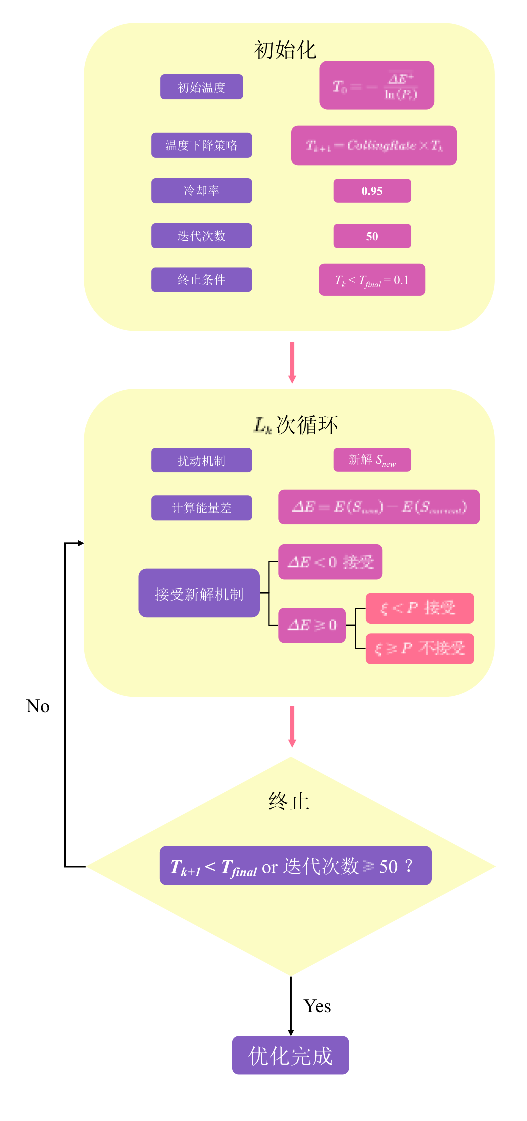
\includegraphics[width=0.5\textwidth]{figures/tuihuo.eps}
		\caption{模拟退火算法流程图}
	\end{figure}
	
	1) 初始化：
	
	通过经验算法生成一个初始温度：
	
	\begin{equation}
	T_0 = -\frac{\overline{\Delta f^+}}{\ln P_r}
	\end{equation}
	
	其中，\(\overline{\Delta f^+}\)为正向（变差）的平均变化，\(P_r\)是初始期望的接受概率。
	
	定义一个温度下降的策略：
	
	\begin{equation}
	T_{k+1} = \text{CoolingRate} \times T_k
	\end{equation}
	
	设定冷却率CoolingRate为0.95，每个温度下进行的迭代次数为50，最大迭代次数为1000，终止条件设置为\(T_k < T_{\text{final}} = 0.1\)。
	
	2) 循环算法：
	
	对每个温度\(T_k\)，执行一次马尔科夫链，即\(L_k\)次循环，通过一个扰动机制在当前解\(S_{\text{current}}\)的基础上产生一个新解\(S_{\text{new}}\)，计算新解与当前解的能量差：
	
	\begin{equation}
	\Delta E = f(S_{\text{new}}) - f(S_{\text{current}})
	\end{equation}
	
	对于最小化问题，根据\textbf{Metropolis准则}判断是否接受新解，即若\(\Delta E < 0\)，则表示新解由于当前解，无条件接受新解。若\(\Delta E \geq 0\)，以一定概率接受，接受概率公式如下：
	
	\begin{equation}
	P = \exp\left(-\frac{\Delta E}{T_k}\right)
	\end{equation}
	
	其中，exp为指数函数，\(T_k\)为当前温度。生成一个在\([0,1)\)区间上均匀分布的随机数\(r\)，比较\(r\)与接受概率\(P\)：
	
	\[
	\begin{cases}
		\text{若 } r < P, & \text{接受新解 } S_{\text{new}} \\
		\text{若 } r \geq P, & \text{保留当前解 } S_{\text{current}}
	\end{cases}
	\]
	
	3) 降温与终止：
	
	完成了当前温度\(T_k\)的\(L_k\)次循环后，检查终止条件\(T_{k+1} < T_{\text{final}}\)，若未满足，则回到循环，在新的温度下继续迭代；若满足，则算法结束，输出找到的历史最优解\(S_{\text{best}}\)。
	
	\subsubsection{得出预测结果}
	
	本文利用MATLAB实现模拟退火算法，优化定价策略，由于篇幅原因，仅展示部分单品结果，全部结果见文件Q3SA.xlsx：
	
	\begin{table}[htbp]
		\centering
		\renewcommand{\arraystretch}{1.5}
		\renewcommand{\heavyrulewidth}{1.2pt}
		\caption{预测结果}
		\begin{tabular}{cccc}
			\hline
			\textbf{单品组合} & \textbf{2021年相关系数} & \textbf{2022年相关系数} & \textbf{2年平均相关系数} \\
			\hline
			上海青螺丝椒(份) & -0.410018296 & -0.903074635 & -0.656546465 \\
			上海青小青菜(份) & -0.426960775 & -0.884997079 & -0.655978927 \\
			云南生菜螺丝椒(份) & -0.468748579 & -0.83800917 & -0.653378874 \\
			上海青云南生菜(份) & -0.429652604 & -0.871453397 & -0.650553 \\
			上海青杏鲍菇(2) & -0.404275203 & -0.894663846 & -0.649469525 \\
			上海青奶白菜(份) & -0.426960775 & -0.86276201 & -0.644861392 \\
			上海青菜心(份) & -0.426960775 & -0.845851263 & -0.636406019 \\
			\hline
		\end{tabular}
		\label{tab:prediction_results}
		\renewcommand{\heavyrulewidth}{0.8pt}
	\end{table}
	
	
	%肖晓伟,肖迪,林锦国,等.多目标优化问题的研究概述[J].计算机应用研究,2011,28(03):805-808+827.
	
\end{document}